\chapter{Evaluation}

This section will investigate the project's findings, any issues encountered during the research and implementation, and the approaches taken to resolve them.

To start, OM2M and OpenMTC will be compared in terms of usability, development of AEs and issues experienced. These would be primarily the team's experiences with development. Then a discussion detailing findings and issues with camera streaming through the OM2M and OpenMTC. Finally, an evaluation on the approaches taken with federations between OpenMTC, OM2M and oneTRANSPORT.

\section{Eclipse OM2M Platform}

\subsection{Usability}

Development for OM2M applications requires a specific version of the Eclipse IDE only. Following the tutorial on installing all the necessary packages for development some of the team ran into OS issues with Windows 10 and had to use Linux Ubuntu 16.04 Desktop or Linux Mint Sylvia 18.3 Virtual Machines to get the development environment set-up. From the team's experience, it was almost impossible to know which OSs will support the required development environment and which will not, out of the box.

Packages used in OM2M were dependent on Java version 7 and would fail with Java version 8. Therefore, it was not possible to take advantage of the new technologies that Java 8 provides, such as the lambda expressions. Members of the team had to modify their Java Runtime Environment (JRE) during set-up as most members' environments had been set up to use a Java 1.8 (Java version 8) platform instead of a Java 1.7 (Java version 7) platform. 

\subsection{Coding}

The code given in the sample plug-in is relatively simple to understand, once the time had been taken. The encapsulation of it made it straightforward to alter it for the needs of the project \ref{om2mpluginstruct}. Although, when a portion of code went misunderstood, the team had to go through many pages of oneM2M documentation to figure out the misunderstanding. The same would be said for portions of written code the team made that did not behave in the way it was intended.

\begin{figure}[H]
  \centering
  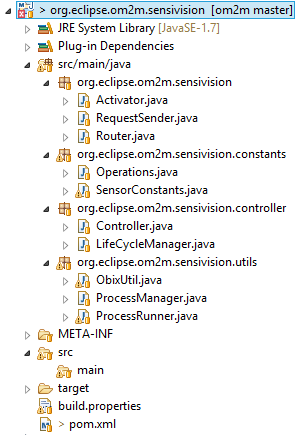
\includegraphics[scale=1]{om2mpluginstructure}
  \caption{OM2M Plug-in Structure}
  \label{om2mpluginstruct}
\end{figure}

Eclipse OM2M does not provide specifications, but rather provides guides on implementing certain elements of the OM2M platform in a specific manner. The team had to resort to using these and documentation from the oneM2M site \cite{onem2mhome}.

Whilst the guides are useful, they do not provide all the information required to completely build a custom OM2M system. Although the technical documents on the site were useful for understanding the core concepts that drive oneM2M, each document was extremely large in length and took multiple reads to fully comprehend. On top of this there were slight nuances with how OM2M works in comparison to how oneM2M states certain elements should be implemented, because of this the team had to experiment with their methodologies until a solution was found.

\subsection{Interface}

As mentioned in the previous chapter, Eclipse OM2M provides a highly intuitive interface (an interactive resource tree visualiser). This interface allows administrators/users of the system to see what is going on in real time and to also interact with it. It is automatically run on OM2M start-up, so by simply navigating to the device in a web browser, users can quickly and easily browse the entire resource tree structure as well as make REST calls without using REST API clients (e.g. Postman or Insomnia) to create HTTP requests on the behalf of users.

The interface is static HTML served by a Jetty web server. Visualising and interactivity is not a result of server-side processes but is the result of JavaScript running client-side.

Due to the OSGi modular approach taking in creating OM2M, it is trivial to enable, disable, or remove such components. In future work, this would allow the team to remove the visualiser if deemed necessary.
 
\subsection{Maven \& Bitbucket Pipelines}

Maven's build and install command was useful to verify that the entire project will build before deploying it on the server and gateway. However, most failures occurred because of the aforementioned Java SE problem.

Bitbucket pipelines also allowed the team to verify whether a commit that was pushed broke the system. In the case of a pushed commit breaking the system, the whole team would be notified would remedy the situation hastily. Most of the time this would not happen as, a commit that breaks the system would not pass the Maven build tests. However, as some of the team occasionally failed to verify with Maven or used a separate IDE, the team was glad that Bitbucket acted as a secondary measure.

\section{OpenMTC Platform}

\subsection{Usability}

Application development for OpenMTC was more accessible than OM2M. Separate Python files were written and then were launched independently from IN and MN and attached to either of them. There was no need to compile or build the project, as it was written in Python (an interpreted language), it was possible to directly change the Python files from the Raspberry Pi, as opposed to OM2M where files were compiled on a separate computer and then copied over to the Raspberry Pi due to its low hardware capabilities.

OpenMTC does not provide a visual interface for managing and visualising the resource structure inside the IN or MN. It only opens a RESTful API. Therefore, a third-party REST API application such as Insomnia\footnote{REST API client https://insomnia.rest/} was required for querying the API.

With the experiences and skills of the team, it was estimated that the task of creating a resource visualisation web interface would not be complicated but this task was outside the scope of this project.

\subsection{HTTPS Issues}

The IN servers as well as InterDigital's oneTRANSPORT were using HTTPS as a communication mechanism. When trying to register an OpenMTC IN-CSE as a RemoteCSE on OM2Ms or oneTRANSPORT's IN-CSE, there were issues validating client SSL certificates from OpenMTC on the server. In an HTTPS communication instantiation, server verification of the client certificate is optional, but OpenMTC forced this check when using HTTPS. The code in figure \ref{https}\footnote{https://github.com/OpenMTC/OpenMTC/blob/d3f33aa1536e9c1039264d2b2f2045d776447745/common/openmtc-oneM2M/src/openmtc\_oneM2M/client/http.py\#L95-L110} shows the code responsible for establishing connection to an IN host via HTTP(S). 

\begin{figure}[H]
  \centering
  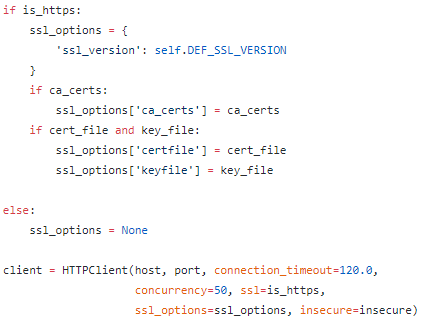
\includegraphics[width=.75\linewidth]{https}
  \caption{Source Code from OpenMTC}
  \label{https}
\end{figure}

To resolve this issue, modifications had to be made to the communication establishment between the client (IN-CSE) and server (other IN-CSE) and remove the parameter that passes the client certificate. Only the client would perform server certificate versification and the server would trust all clients connecting. 

In the figure \ref{https}, \lstinline{HTTPclient} called from an OpenMTC IN-CSE trying to establish a connection with another IN-CSE. Passed in to the function are parameters for locating the server (\lstinline{host} and \lstinline{port}) as well as \lstinline{ssl_options}. Part of the SSL options are the client certificates passed to the server. Server-side verification is an optional step and by removing this step a valid connection can be established. 

\section{Video Streaming Through oneM2M}

This section will evaluate the implementations of video streaming as well as giving information to the client about future work in this area.

\subsection{OM2M}

Disabling console logging for the MN-CSEs and IN-CSEs allowed the processing of image data to be faster, resulting in a higher frame rate at a higher quality. The stream was running at around 5 frames per second which resulted in the live video feed not being fluid.

Parsing the data image from Python to Java proved to be the main issue which resulted in the low frame rate of the stream. Although this simplified the development process for the team it effected the performance of the video stream

Java's virtual machine and heavy XML document structure was also an issue when interacting with the camera data.

Future work with OM2M to improve its effectiveness should ideally be on micro controllers with greater hardware capabilities, be only interacting with the Raspberry Pi through Java libraries and using a JSON structure for simplified parsing. 

\subsection{OpenMTC}

Compared to OM2M, video streaming using OpenMTC was much more successful. This was likely due to lower overheads of the Python runtime environment when compared to the Java Virtual Machine, and the simpler architecture of OpenMTC in general.

While OM2M managed to achieve 5 frames per second, OpenMTC could broadcast 20 frames per second. This is a significant improvement, it is the difference between a slide show, and somewhat fluid motion.

This was mainly due to the fact that the image data did not require any parsing between programming languages as OpenMTC and the Raspberry Pi scripts were all written in Python. OpenMTC uses the JSON structure for serialization which requires less processing and parsing then XML used by OM2M.    

\subsection{Live Video Feed Website}

The live video feed website was only made as a testing platform to visualize the data being sent other oneM2M system. It was not built with scalability or future usability in mind.

Every web client that opened the video feed using a browser would generate 20 requests a second to the In-CSE requesting the latest data from the video feed. For example, 10 clients would generate 200 requests per second that could lead to DDOS (Distributed Denial of Services) being performed on the public facing IN-CSE server.

If the client wants to reproduce this project, the team suggests taking advantage of the subscription and notification mechanisms implemented in most oneM2M platforms described in section \ref{sec:sub}.

The web server hosting the video feed would subscribe to the IN-CSE telling it to update when a new video frame is available. The IN-CSEs security services can authenticate and authorize the application requesting the subscription. Once an image frame is available it would notify the web server with the data that can be displayed to the user.

\section{oneM2M Platform Federation}

In the context of the implementation, the team did not achieve mutual federation between service providers. Between open source implementations (OM2M and OpenMTC), only one way federation was established due to the \lstinline{ValueError: 28 is not a valid ResourceType} error. With regards to oneTRANSPORT, data was federated while their platform required extra authentication that will be explained in this section.  

\subsection{OM2M and OpenMTC}

Both IN-CSEs from OM2M and OpenMTC have a list of Supported Resource Types (SRT) mentioned in listing \ref{lst:srt} OpenMTC's SRTs is subset of OM2Ms SRTs and as it can be seen in listing \ref{lst:srt}, OpenMTC is missing the resource type 28 for flexible containers. Therefore, a two-way federation was not possible due to the error \lstinline{ValueError: 28 is not a valid ResourceType}.\\

\begin{lstlisting}[caption={OM2M and OpenMTC supported resource types}, label={lst:srt}]
OM2M:    1 2 3 4 5 9 14 15 16 17 23 28
OepnMTC: 1 2 3 4 5 9 14 15 16 17 23
\end{lstlisting}

For mutual federation to occur, both IN servers must implement the exact same set of resource types (SRTs) otherwise only one-way federation will be possible.

\subsection{OpenMTC and oneTRANSPORT}

Because of oneTRANSPORTs security design, it required specific headers to be present in every request when communicating with its IN-CSE. This therefore required a modification in the underlying HTTP communication of the platform choice. Using OpenMTC it was easy to locate the section of the code that needed modification (figure \ref{headers}).

\begin{figure}[H]
  \centering
  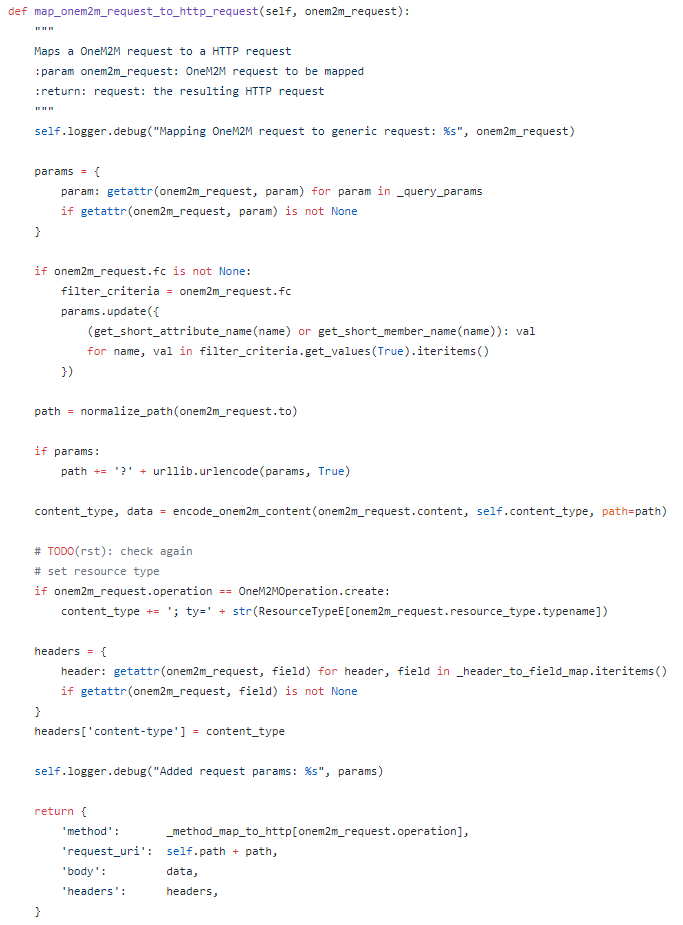
\includegraphics[width=.93\linewidth]{headers}
  \caption{Header Injection Location in OpenMTC}
  \label{headers}
\end{figure}

When translating oneM2M requests to HTTP requests, the translator displayed in figure \ref{headers} could have the functionality for custom headers added so that oneTRANSPORT can authenticate and authorize  the IN used. 

This would only be necessary to access oneTRANSPORT data. But, because the OpenMTC IN-CSE did not implement any custom requests authentication, oneTRANSPORT could successfully query data without the previous changes.

\clearpage
